\documentclass[a4paper]{article}

\usepackage{fontspec}
\usepackage{polyglossia}

\setmainlanguage{russian}
\setotherlanguages{english}

% download "Linux Libertine" fonts:
% http://www.linuxlibertine.org/index.php?id=91&L=1
\setmainfont{Linux Libertine O} % or Helvetica, Arial, Cambria
% why do we need \newfontfamily:
% http://tex.stackexchange.com/questions/91507/
\newfontfamily{\cyrillicfonttt}{Linux Libertine O}





\usepackage{amsmath} % Математические окружения AMS
\usepackage{amsfonts} % Шрифты AMS
\usepackage{amssymb} % Символы AMS
\usepackage{mathtext} % Русские буквы в фомулах
\usepackage{graphicx} % Вставить pdf- или png-файлы

\usepackage{color}
\usepackage{bbold}

\usepackage{booktabs}

\usepackage{mathrsfs} % Красивый шрифт

\usepackage{longtable}  % Длинные таблицы
\usepackage{multirow} % Слияние строкв таблице

\usepackage{indentfirst} % Отступ в первом абзаце.
\usepackage{tikz}

\newcommand*{\hm}[1]{#1\nobreak\discretionary{}%
            {\hbox{$\mathsurround=0pt #1$}}{}}

\usepackage{verbatim}

\DeclareMathOperator{\sgn}{\mathop{sgn}}
\DeclareMathOperator{\card}{\mathop{card}}

\usepackage{enumitem}


\usepackage{fancyhdr}
\usepackage[margin=1in]{geometry}


\AddEnumerateCounter{\asbuk}{\russian@alph}{щ} % для списков с русскими буквами
\setlist[enumerate, 2]{label=\asbuk*),ref=\asbuk*}


\pagestyle{fancy} \makeatletter \fancyhead[L]{\footnotesize ICEF, 2016/17, «Mathematics for Economists»}

\makeatletter
\newcommand*{\rom}[1]{\expandafter\@slowromancap\romannumeral #1@}
\makeatother

 \begin{document}
 \begin{center}
 {\Large{Конспект лекции 17.11.16}}
 \end{center}
  \begin{center}
 {\large{Фомина Александра}}
 \end{center}
 \par {\bf\underline{Мотивация.}} $\sigma$-алгебра - это способ описать наделенность информации: есть рациональный агент и список событий, про которые агент {\it точно} знает, произошли они или нет.\\
 \par {\bf\underline{Упражнение 1.}} Подбрасывают кубик два раза. Случайная величина $X_1$ - сколько выпало в первый раз, случайная величина $X_2$ - сколько выпало во второй раз. Винни Пух знает результаты обоих подбрасываний. Джеймс Бонд знает результат только второго подбрасывания. Если $\mathcal{F}_W$ и $\mathcal{F}_J$ - это списки событий, которые точно различают Винни Пух и Джеймс Бонд соответственно, то
\begin{enumerate}
\item $\mathcal{F}_J\subset\mathcal{F}_W$;
\item Примеры события $A$, $A\in\mathcal{F}_W$, $A\not\in\mathcal{F}_J$: $A=\{X_1=4\}\in\mathcal{F}_W$, $A=\{X_1=4\}\not\in\mathcal{F}_J$;
\par  Примеры события $B$, $B\in\mathcal{F}_W$, $B\in\mathcal{F}_J$: $B=\{X_2>4\}\in\mathcal{F}_W$, $B=\{X_2>4\}\in\mathcal{F}_J$.\\
\end{enumerate}
\par {\bf\underline{Упражнение 2.}} Тот же эксперимент, что и в Упражнении 1, те же $\mathcal{F}_W$ и $\mathcal{F}_J$. Какова мощность множества (cardinality) $\mathcal{F}_W$ и $\mathcal{F}_J$?\\
\par Пусть $\Omega$ - множество исходов. Тогда $\Omega=36$, т.к. всего 36 элементарных события, которые нельзя разбить на более мелкие события.\\
\[\begin{tabular}{c|ccc}
\hline
$X_1\setminus X_2$&1&2&\dots\\
\hline
1&(1,1)&(1,2)&\dots\\
2&(2,1)&(2,2)&\dots\\
\vdots&\vdots&\vdots&$\ddots$\\
\end{tabular}\]
\par Большие события получаются путем объединения маленьких событий. Например: \[\{X=4\}=\{X_1=4,X_2=1\}\cup\{X_1=4,X_2=2\}\cup\{X_1=4,X_2=3\}\cup\dots\]
 \[\begin{tabular}{c|cccccc}
\hline
$X_1\setminus X_2$&1&2&3&4&5&6\\
\hline
1&-&-&-&-&-&-\\
2&-&-&-&-&-&-\\
3&-&-&-&-&-&-\\
4&+&+&+&+&+&+\\
5&-&-&-&-&-&-\\
6&-&-&-&-&-&-\\
\end{tabular}\]
 \par Так как всего в таблице 36 клеток, в каждой из который может стоять либо "$+$"\, либо "$-$"\ , то всего может быть $2^{36}$ вариантов. Следовательно, $\card \mathcal{F}_W=2^{36}$.\\
 \par Для Джеймса Бонда $\{X_2=4\}$ не разбивается на более элементарные события $\Rightarrow$ у него 6 элементарных события, то есть  $\card\mathcal{F}_J=2^6$.\\
 \begin{itemize}
  \item Если агент знает, что $A\in\mathcal{F}$ и $B\in\mathcal{F}$, то он знает, что $A^c\in\mathcal{F}$, $A\cap B\in\mathcal{F}$, $A\cup B\in\mathcal{F}$.\\
 \item $\varnothing$ не происходит никогда, $\Omega$ происходит всегда $\Rightarrow\;\varnothing\in\mathcal{F}$, $\Omega\in\mathcal{F}$.
 \end{itemize}
 \par {\bf\underline{Определение.}} $\mathcal{F}$ -- $\sigma$-алгебра, если
 \begin{enumerate}
 \item $\varnothing,\Omega\in\mathcal{F}$;
 \item если взять счётное (countable) количество событий из $\mathcal{F}$ и выполнить любые операции \\($\cdot\cup\cdot,\cdot\cap\cdot,\cdot\setminus\cdot,\cdot^c$), то в результате получится событие из списка $\mathcal{F}$.
\end{enumerate}
 \par {\bf\underline{Альтернативное определение.}} $\mathcal{F}$ -- $\sigma$-алгебра, если
 \begin{enumerate}
 \item $\Omega\in\mathcal{F}$;
 \item если $A\in\mathcal{F}$, то и $A^c\in\mathcal{F}$;
 \item если $A_1,A_2,A_3,\dots\in\mathcal{F}$, то $\cup_{i=1}^{\infty}A_i\in\mathcal{F}$.\\
\end{enumerate}
 \par {\bf\underline{Определение.}} $\sigma(B,C)$ -- минимальная $\sigma$-алгебра, содержащая события $B$ и $C$.\\
\par {\bf\underline{Упражнение 3.}} $\Omega=\Re$, $A=[-10;-5]$, $B=[-7,0)$. Найти: $\sigma(A)$, $\sigma(A,B)$.
\[\sigma(A)=\{\varnothing,\Re,[-10;-5],(-\infty;-10)\cup(-5;+\infty)\}\]
\[\sigma(A,B)=\{\varnothing,\Re,[-10;-5],[-7;0),[-10;0),(-\infty;-10)\cup(-5;+\infty),(-\infty;-7)\cup[0;+\infty),(-\infty;-10)\cup[0;+\infty),\]
\[[-7;-5],(-\infty,-7)\cup(-5;+\infty),[-10;-7],(-\infty;-10)\cup(-7,+\infty),[-5,0),(-\infty;-5)\cup[0,+\infty),\] \[(-\infty;-10)\cup(-7;-5)\cup[0;+\infty),(-10,-7)\cup(-5;0]\}\]
\par Так как $-10,\;-7,\;-5$ и 0 делят числовую прямую на 4 "куска"\ , то в $\sigma(A,B)$ всего $2^4$ элементов.\\
\begin{center}{\large Случайные величины}\end{center}
\par {\bf\underline{Определение (интуитивное).}} Случайная величина $X$ называется измеримой относительно $\sigma$-алгебры $\mathcal{F}$, если информации в $\mathcal{F}$ достаточно, чтобы определить, чему равно $X$.\\
\par {\bf\underline{Определение (формальное).}} Случайная величина $X$ называется измеримой относительно $\sigma$-алгебры $\mathcal{F}$, если $\forall t$ событие $\{X\leq t\in\mathcal{F}\}$.\\
\par {\bf\underline{Упражнение 4.}}
\[\begin{tabular}{*{5}{c}}
\toprule
$\Omega$&a&b&c&d\\
\midrule
X&1&1&2&2\\
Y&1&3&3&1\\
\bottomrule
\end{tabular}\]\\
\[\mathcal{F}=\{\varnothing,\Omega,\{a,c\},\{b,d\}\}\]
\[\mathcal{H}=\{\varnothing,\Omega,\{a,d\},\{b,c\}\}\]
\par a) Является ли $X$ измеримой случайно величиной относительно $\mathcal{F}$? Нет, так как, если произошло а, мы не можем отличить а от с, потому что у них разные значения. Значит, мы не знаем, чему равна $X$.\\
\par b) Является ли $Y$ измеримой случайно величиной относительно $\mathcal{F}$? Нет.\\
\par c) Является ли $X$ измеримой случайно величиной относительно $\mathcal{H}$? Нет.\\
\par d) Является ли $Y$ измеримой случайно величиной относительно $\mathcal{F}$? Да.\\
 \par {\bf\underline{Обозначение.}} $X,\;Y$ -- случайные величины. Тогда $\sigma(X,Y)$ -- минимальная $\sigma$-алгебра, содержащая все события вида $\{X\leq t\}$ и $\{Y\leq t\}$.\\
\par {\bf\underline{Упражнение 5.}}
\[\begin{tabular}{*{5}{c}}
\toprule
$\Omega$&a&b&c&d\\
\midrule
X&1&1&2&2\\
Y&1&3&3&1\\
W&7&1&2&2\\
\bottomrule
\end{tabular}\]
\par a) Найти явно $\sigma(X)$. \[\sigma(X)=\{\varnothing,\Omega,\{a,b\},\{c,d\}\}\]
\par b) Определить, сколько событий входит в $\sigma(X,Y)$.
\par Если мы знаем $X$ и $Y$, мы знаем, что произошло: a, b, c или d. Следовательно, $\card \sigma(X,Y)=2^4$.\\
\par c) Найти явно $\sigma(W)$. \[\sigma(W)=\{\varnothing,\Omega,\{a\},\{b\},\{c,d\},\{a,b\},\{a,c,d\}\}\]
\par {\bf\underline{Определение (интуитивное).}} Условное матожидание:
\begin{enumerate}
\item $E(Y|\mathcal{F})$ -- случайная величина;
\item $E(Y|\mathcal{F})$ -- наилучший (с т. з. минимизации ожидаемого квадрата ошибки) прогноз $Y$, сделанный агентом, различающим события из $\mathcal{F}$.
\end{enumerate}
 \par {\bf\underline{Обозначение.}} $E(Y|X)=E(Y|\sigma(X))$\\
\par {\bf\underline{Упражнение 6.}}  Кубик подбрасывается два раза. $X_i$ - результат $i$-го подбрасывания. $\mathcal{F}_J~=~\sigma(X_2)$.\\
\par a) Найти $E(X_2|\mathcal{F}_J)$. $E(X_2|\mathcal{F}_J)=X_2$;\\
\par b) Найти $E(X_2^2|\mathcal{F}_J)$. $E(X_2^2|\mathcal{F}_J)=X_2^2$;\\
\par c) Найти $E(X_1|X_2)$. Так как $X_1$ и $X_2$ независимы, то знание про $X_2$ бесполезно. Следовательно, $E(X_1|X_2)=E(X_1)=3,5$;\\
\par d) Найти $E(X_1+X_2|X_2)$. $E(X_1+X_2|X_2)=E(X_1|X_2)+E(X_2|X_2)=3,5+X_2$.\\
\begin{center}{\large Свойства матожидания}\end{center}
\par Если $X$ и $Y$ -- случайные величины, $E(X)$ и $E(Y)$ существуют, a и b -- константы, $\mathcal{F},\;\mathcal{H}$ -- $\sigma$-алгебры, $\mathcal{F}\leq\mathcal{H}$:
\begin{enumerate}
\item $E(aX+bY|\mathcal{F})=aE(X|\mathcal{F})+bE(Y|\mathcal{F})$.
\item Если $X$ и $\mathcal{F}$ независимы, то $E(X|\mathcal{F})=E(X)$.
\item Если $X$ измерима относительно $\mathcal{F}$ и $g(\;)$ -- кусочно-непрерывная функция, то $E(g(X)|\mathcal{F})~=~g(X)$.
\item Если $\mathcal{F}=\{\varnothing,\Omega\}$, то $E(X|\mathcal{F})~=~E(X)$.
\item $E(E(X|\mathcal{F}))=E(X).$
\item Если $\mathcal{F}\leq\mathcal{H}$, то $E(E(X|\mathcal{H})=E(X|\mathcal{F})$ и $E(E(X|\mathcal{H})=E(X|\mathcal{F})$.
\item Неравенство Йенсен: если $f$ -- выпуклая, то $E(f(X)|\mathcal{F})\geq f(E(X|\mathcal{F}))$.\\
\par Дополнительные понятия:\\
 \par {\bf\underline{Определение.}} $A$ -- событие, $\mathbb{1}_A=\begin{cases}1,&\text{если $A$ произошло}\\
 0,&\text{если $A$ не произошло}\end{cases}$ -- индикатор $A$, $E(\mathbb{1}_A)=P(A)$. Тогда $P(A|\mathcal{F})=E(\mathbb{1}_A|\mathcal{F})$.\\
  \par {\bf\underline{Определение.}} Условная дисперсия: $Var(X|\mathcal{F})=E(X^2|\mathcal{F})-(E(X|\mathcal{F}))^2$.\\
  \par Свойства условной дисперсии:
  \item Если $g$ -- кусочно-непрерывная функция и $X$ измерима относительно $\mathcal{F}$, то $Var(g(X)|\mathcal{F})=0$.
  \item Теорема Пифагора: $Var(X)=Var(E(X|\mathcal{F}))+E(Var(X|\mathcal{F}))$.
\end{enumerate}
\par Геометрический взгляд:
\[\begin{tabular}{ccc}
9 класс&&1 курс магистратуры\\
a, b -- векторы&&\\
$cos(a,b)=\cfrac{\langle a,b\rangle }{|a|\cdot|b|}$&$\longrightarrow$&$\cfrac{Cov(X,Y)}{\sqrt{Var(X)Var(Y)}}=corr(X,Y)$
\end{tabular}\]
\par $\langle a,b\rangle\;\longleftrightarrow\;Cov(X,Y)$
\par $|a|^2=\langle a,a\rangle\;\longleftrightarrow\;Cov(X,Y)=Var(X)$
\par $|a|\;\longleftrightarrow\sigma_X$\\
\par Если $X\perp Y$ $(Cov(X,Y)=0)$, то $Var(X)+Var(Y)=Var(X+Y)$ (т. Пифагора).\\

\[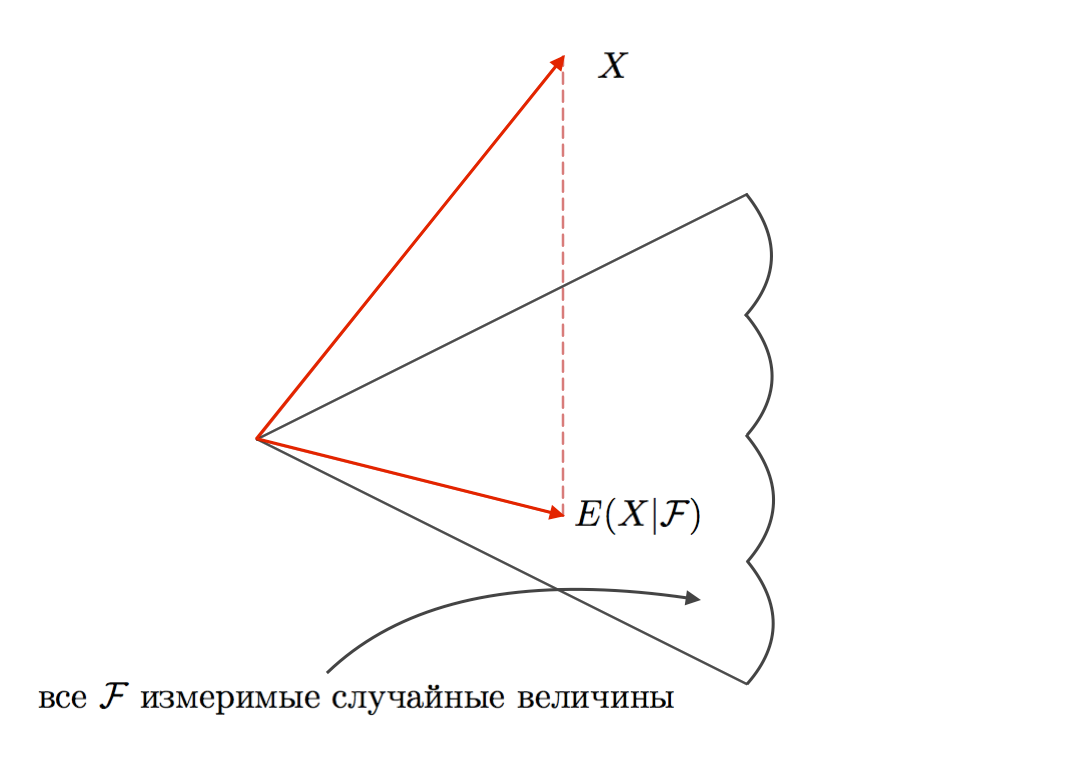
\includegraphics[width=0.75\linewidth]{01_projection.png}\]

\par $Var(X)=Var(E(X|\mathcal{F}))+Var(X-E(X|\mathcal{F}))$\\
\par {\bf\underline{Определение (формальное).}} Если $E(X)$ существует, то $E(X|\mathcal{F})$ -- это случайная величина, которая
\begin{enumerate}
\item $\mathcal{F}$ измерима;
\item $E(X)=E(E(X|\mathcal{F}))$;
\item $X-E(X|\mathcal{F})\;\perp$ любой $\mathcal{F}$ измеримой случайной величине, т.е. $Cov(X-E(X|\mathcal{F}),Z)=0$ для любой случайной величины $Z$, являющейся $\mathcal{F}$ измеримой.\\
\end{enumerate}
\par {\bf\underline{Определение.}} Случайная величина $W$ называется условным матожиданием $E(X|\mathcal{F})$ если
\begin{enumerate}
\item $W$ является $\mathcal{F}$ измеримой;
\item $E(X)=E(W)$;
\item $Cov(X-W,Z)=0$ для любой $\mathcal{F}$ измеримой $Z$.\\
\end{enumerate}
\par {\bf\underline{Упражнение 7.}}
\[\begin{tabular}{*{5}{c}}
\toprule
$\Omega$&a&b&c&d\\
\midrule
X&1&1&2&2\\
Y&1&3&3&1\\
\text{Вероятность}&0,1&0,2&0,3&0,4\\
\bottomrule
\end{tabular}\]
\par Найти $Var(X|\sigma(Y))$.
\[Var(X|\sigma(Y))=E(X^2|Y)-(E(X|Y))^2=\begin{cases}\cfrac{17}5-\left(\cfrac95\right)^2,&\text{если}\; Y=1\\
\cfrac{14}5-\left(\cfrac85\right)^2,&\text{если}\;Y=3\end{cases}=\left(\cfrac{17}5-\left(\cfrac95\right)^2\right)\cdot\mathbb{1}_{Y=1}+\left(\cfrac{14}5-\left(\cfrac85\right)^2\right)\cdot\mathbb{1}_{Y=3}\]
\[E(X|Y=1)=1\cdot\cfrac{0,1}{0,1+0,4}+2\cdot\cfrac{0,4}{0,1+0,4}=\cfrac95\]
\[E(X|Y=3)=\cfrac85\]
\[E(X^2|Y=1)=\cfrac{17}5\]
\[E(X^2|Y=3)=\cfrac{14}5\]

\end{document}
